\chapter{Thermal Radiation Sensing Concepts for Nuclear Systems}
\label{ch:thermal_sensing}

\section{Introduction}

In addition to the direct detection approaches explored in the preceding chapters, indirect methods of radiation sensing, those that infer radiation fields from their thermal signatures, represent an alternative pathway for monitoring nuclear environments.  Within the materials-to-systems hierarchy that organizes this dissertation, thermal sensing occupies the conceptual bridge between the materials and device investigations of Chapters~\ref{ch:CsFAPbI}--\ref{ch:perovskite_detectors} and the digital electronics instrumentation of Chapters~\ref{ch:digital_electronics}--\ref{chap:fpga_benchmark}: it addresses a system-level sensing function without relying on either semiconductor detector materials or active electronic components in the radiation field.  This chapter describes the investigation of two such concepts: the Optical Fiber-Based Gamma Thermometer (OFBGT) and the Optical Fiber-Based Neutron Dosimeter (OFBND).  Both devices exploit the temperature differential that arises when ionizing radiation deposits energy in a thermally isolated material, and both rely on distributed fiber-optic temperature sensing to measure that differential.  Of the two concepts, the OFBGT reached the experimental validation stage, while the OFBND remains a simulation-based design study.

The OFBGT was originally conceived and developed by Birri~\cite{Birri2021Dissertation} at The Ohio State University.  The present work extends that effort to a new sensor design intended for deployment in the Central Irradiation Facility (CIF) of the Ohio State University Research Reactor (OSURR), carried out in partnership with Luna Innovations~\cite{LunaDOE2024}.  The author's contribution centered on executing and validating thermal simulations of the redesigned OFBGT using analytical models previously established by Birri, as well as extending those models to predict the performance of a proposed neutron-sensitive variant, the OFBND.  The simulation methodology, calculational results, and implications for the experimental campaign are presented in the sections that follow.

\section{Gamma Heating and the Gamma Thermometer Principle}
\label{sec:gamma_heating}

When a material is placed in a mixed radiation field inside a reactor core, gamma rays interact with the material primarily through the photoelectric effect, Compton scattering, and pair production.  These interactions transfer kinetic energy to secondary electrons, which subsequently deposit that energy locally as heat through ionization and excitation of the lattice.  The volumetric rate at which energy is deposited, $Q'''$ (W/m$^3$), depends on the gamma-ray flux, the energy spectrum of the gamma-ray field, and the mass energy-absorption coefficient of the target material.

A gamma thermometer exploits this heating effect by measuring the temperature difference, $\Delta T$, that develops between a thermally insulated internal mass, referred to here as the thermal mass or insulating tube, and an outer metallic sheath that is in thermal contact with the reactor coolant.  Because the insulating gas gap between the thermal mass and the sheath represents the dominant thermal resistance, the temperature within the thermal mass is elevated relative to the sheath.  When the sensor is calibrated by applying a known electrical power to an internal heating wire, a relationship between the linear power density $q'$ and $\Delta T$ is established.  During reactor operation, the measured $\Delta T(z)$ at each axial position $z$ can then be converted to the local $q'(z)$, and hence to the local gamma-ray dose rate~\cite{Birri2021Dissertation, Birri2020IEEE}.

\subsection{Optical Frequency Domain Reflectometry}

The temperature sensing modality employed in both the OFBGT and OFBND is optical frequency domain reflectometry (OFDR).  In OFDR, a tunable laser is swept in wavelength and coupled into a sensing fiber.  The backscattered Rayleigh signal, or the reflected signal from fiber Bragg gratings (FBGs) inscribed along the fiber, is interfered with a reference signal to produce a spatial map of spectral shift along the fiber.  A shift in the reflected spectrum at a given location is linearly related to the local temperature change.  Phase-shifted, continuously written (PSC) type~II FBGs, inscribed by ultrafast laser pulses, were chosen for this application because of their demonstrated radiation hardness and thermal stability at elevated temperatures~\cite{Birri2021Dissertation}.

\section{Optical Fiber-Based Gamma Thermometer Design}
\label{sec:ofbgt_design}

\subsection{Cross-Sectional Geometry}

A generalized cross-section of the OFBGT active sensing region is shown in Figure~\ref{fig:ofbgt_xsec}.  The central element is a repurposed four-hole thermocouple-wire electrical insulator tube composed of 80\% mullite and 20\% silica.  Two of the four holes carry optical fibers that measure the temperature of the thermal mass; the remaining two holes carry a nichrome heating wire that forms a loop for calibration purposes.  When a known current is passed through the heating wire, a known $q'$ is generated, establishing the calibration relationship between $q'$ and $\Delta T$.

\begin{figure}[htbp]
    \centering
    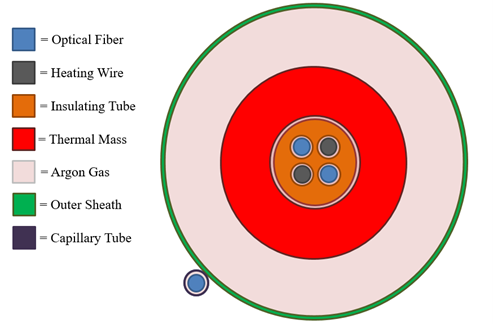
\includegraphics[width=0.6\textwidth]{figures/OFBGT_XSec.png}
    \caption[Cross-sectional view of the OFBGT.]{Cross-sectional view of the optical fiber-based gamma thermometer, showing the insulating tube/thermal mass, optical fibers, heating wire, argon gas gap, and nested outer sheath tubes.  Adapted from the OFBGT Simulation Response Document~\cite{SimReport2023}, p.~2.}
    \label{fig:ofbgt_xsec}
\end{figure}

The insulating tube/thermal mass is surrounded by an argon gas gap at atmospheric pressure (760~mmHg).  Argon was selected for its chemical inertness and well-characterized thermal conductivity ($\kappa_G = 22.6$~mW/(m$\cdot$K) at room temperature).  Because of its low thermal conductivity, the gas gap constitutes the dominant thermal resistance in the radial heat transfer path, making the temperature distribution within the thermal mass nearly uniform.

Two nested aluminum 6061 tubes form the outer sheath.  The inner nested tube has two grooves machined into its outer surface, each containing an optical fiber that senses the sheath temperature.  The temperature difference $\Delta T(z) = T_\mathrm{fiber,inner}(z) - T_\mathrm{fiber,outer}(z)$ between the fibers in the thermal mass and those in the outer sheath is the principal measurement quantity of the OFBGT.

\subsection{Axial Layout}

An overall view of the OFBGT design as configured for the OSURR is shown in Figure~\ref{fig:ofbgt_overall}.  The sensor has three regions in the axial direction.  The bottom-most region is the active sensor region, where the thermal mass, the gas gap, and the outer sheath are present.  The active sensor length was approximately 24~inches (61~cm), constrained by the longest available continuous length of the mullite insulator.  The bottom of the OFBGT is welded shut to maintain the inert argon atmosphere.  Glass disc spacers keep the thermal mass centered within the sheath.

\begin{figure}[htbp]
    \centering
    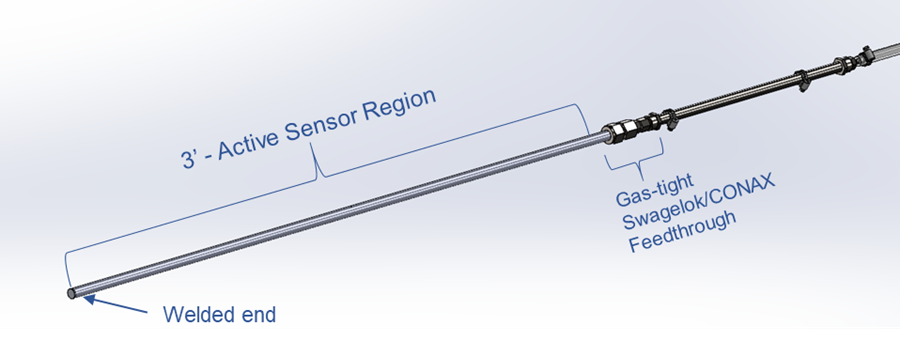
\includegraphics[width=0.6\textwidth]{figures/overall_OFBGT.png}
    \caption[Overall view of the OFBGT.]{Overall view of the OFBGT design for the OSURR, showing the active sensor region, the gas-tight Swagelok/CONAX feedthrough, and the welded end.  Adapted from the OFBGT Simulation Response Document~\cite{SimReport2023}, p.~4.}
    \label{fig:ofbgt_overall}
\end{figure}

\begin{figure}[htbp]
    \centering
    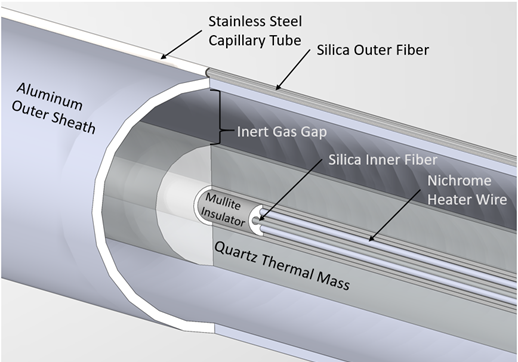
\includegraphics[width=0.6\textwidth]{figures/ofbgt_cutaway.png}
    \caption[Internal view of the OFBGT active sensor region.]{Internal view of the active sensor region of the OFBGT, showing the mullite insulator, nichrome heater wire, silica optical fibers, inert gas gap, and aluminum outer sheath.  Adapted from the OFBGT Simulation Response Document~\cite{SimReport2023}, p.~4.}
    \label{fig:ofbgt_internal}
\end{figure}

\section{Optical Fiber-Based Neutron Dosimeter Concept}
\label{sec:ofbnd_concept}

The OFBND extends the gamma thermometer concept to neutron fields by replacing the mullite insulator with borosilicate glass.  Borosilicate glass contains boron-10, which has a large thermal-neutron absorption cross-section ($\sigma_B \approx 755$~barns for natural boron).  When a thermal neutron is absorbed by $^{10}$B, the resulting $^{10}$B(n,$\alpha$)$^{7}$Li reaction releases charged particles whose kinetic energy is deposited locally as heat:
\begin{equation}
    \langle Q_\alpha^B + Q_{Li}^B \rangle = 3.75 \times 10^{-13}~\text{J/reaction} \, .
    \label{eq:boron_Q}
\end{equation}
where the angle brackets denote averaging over the two branches of the reaction.  The volumetric energy deposition rate in the borosilicate thermal mass is then
\begin{equation}
    Q''' = N_B \, \sigma_B \, \varphi \, \langle Q_\alpha^B + Q_{Li}^B \rangle
    \label{eq:Qppp_neutron}
\end{equation}
where $N_B$ is the boron number density and $\varphi$ is the thermal neutron flux.

The OFBND is geometrically similar to the OFBGT but uses a smaller-diameter thermal mass.  Whereas the OFBGT employs a 1/8-inch (3.175~mm) OD mullite tube, the OFBND uses a 1/16-inch (1.5875~mm) OD borosilicate glass tube.  The smaller diameter was driven by the availability of borosilicate capillary tubing.  The neutron-sensitive thermal mass is to be deployed in the Auxiliary Irradiation Facility (AIF) of the OSURR, where the thermal neutron flux is $6.0 \times 10^{12}$~n~cm$^{-2}$s$^{-1}$.

By placing a standard gamma-sensitive OFBGT and a neutron-sensitive OFBND at adjacent positions in the reactor, it becomes possible in principle to separate the neutron and gamma contributions to the local dose rate.  The neutron-to-gamma heating ratio in the borosilicate glass thermal mass is approximately 4:1 at the thermal neutron fluxes encountered in the AIF, making the OFBND substantially more responsive to neutrons than to gamma rays~\cite{SimReport2023}.

\section{Simulation Methodology}
\label{sec:simulation_methodology}

\subsection{Analytical Thermal Model}

The thermal response of the OFBGT and OFBND was predicted using an analytical model originally developed by Birri~\cite{Birri2020IEEE, Birri2021Dissertation}.  The model treats the sensor as a series of concentric cylindrical regions, thermal mass, gas gap, and outer sheath, with azimuthal symmetry assumed.  Deviations from azimuthal symmetry due to the heating wire and optical fiber holes are small and were neglected.

Under the assumption that the linear power density $q'$ is axially uniform and the outer sheath surface temperature $T(r_{So}, z)$ is axially constant, the temperature difference between the fiber location in the thermal mass and the outer sheath surface is
\begin{equation}
    \Delta T(z) = T(r_f, z) - T(r_{So}, z) = q' \, R_{r_f}^{r_{So}}
    \label{eq:deltaT}
\end{equation}
where $q' = Q''' \pi r_{TM}^2$ is the linear power density for the sensor, $r_f$ is the radial position of the optical fiber within the thermal mass, $r_{TM}$ is the outer radius of the thermal mass, and $R_{r_f}^{r_{So}}$ is the thermal resistance from the fiber location to the outer sheath surface:
\begin{equation}
    R_{r_f}^{r_{So}} = \frac{1}{2\pi} \left[ \frac{\displaystyle 1 - \frac{r_f^2}{r_{TM}^2}}{2\kappa_{TM}} + \frac{\displaystyle \ln\left(\frac{r_{Si}}{r_{TM}}\right)}{\kappa_G} + \frac{\displaystyle \ln\left(\frac{r_{So}}{r_{Si}}\right)}{\kappa_S} \right]
    \label{eq:thermal_resistance}
\end{equation}
Here $\kappa_{TM}$, $\kappa_G$, and $\kappa_S$ are the thermal conductivities of the thermal mass, gas gap, and sheath, respectively, and $r_{Si}$ and $r_{So}$ are the inner and outer radii of the outer sheath.

This expression is exact for the case of axially constant $q'$ and axially constant outer sheath temperature.  In a reactor, however, $q'(z)$ varies axially following the neutron flux profile.  To characterize the resulting error, a modulation transfer function (MTF) formalism was employed.

\subsection{Modulation Transfer Function}
\label{sec:MTF}

The concept of a modulation transfer function, borrowed from optical imaging theory, was applied to the OFBGT by Palmer and Blue~\cite{Palmer2018}.  When the volumetric energy deposition $q'''(z)$ varies sinusoidally with spatial frequency $k = 2\pi/\lambda$, axial diffusion of thermal energy in the thermal mass, gas gap, and sheath causes the measured $\Delta T(z)$ to be attenuated (modulated) relative to the true $q'''(z)$ distribution.  During calibration with a spatially uniform heat source ($k = 0$), this axial diffusion does not occur.  The normalized MTF quantifies the ratio of the sensor response at spatial frequency $k$ to the response at $k = 0$:
\begin{equation}
    \mathrm{MTF}_\mathrm{norm}(k) = \frac{\mathrm{MTF}(k)}{\mathrm{MTF}(k=0)} = \frac{R_{TM}(r_f)\big|_k}{R_{TM}(r_f)\big|_{k=0}}
    \label{eq:MTF_norm}
\end{equation}
where $R_{TM}(r_f)\big|_k$ is a function of the modified Bessel functions $I_0$ and $K_0$ evaluated at the boundaries of the three regions, determined by solving a $5 \times 5$ matrix equation that enforces continuity of temperature and heat flux at the interfaces~\cite{Birri2020IEEE, SimReport2023}.

A value of $\mathrm{MTF}_\mathrm{norm}$ close to unity indicates that the OFBGT faithfully reproduces the axial variation in $q'''(z)$ at that spatial frequency.  As $k$ increases, the MTF decreases, indicating a loss of axial resolution.

\subsection{Computational Implementation}

Two computational implementations of the analytical model were used:

\begin{enumerate}
    \item \textbf{Python model.}  A point calculation based on Equations~\ref{eq:deltaT}--\ref{eq:thermal_resistance} was implemented in Python to compute $\Delta T$ at the axial location of maximum $q'$.  This model assumed constant (room-temperature) thermal conductivities.
    \item \textbf{MATLAB model.}  A more comprehensive model was implemented in MATLAB that solved the matrix equation for the temperature distribution $T(r,z)$ throughout the entire sensor, iteratively updating the temperature-dependent thermal conductivities of the argon gas gap, the thermal mass, and the outer sheath at each axial and radial position until convergence was achieved.  The MATLAB model also computed the normalized MTF as a function of spatial frequency $k$.
\end{enumerate}

The MATLAB code iterated on the thermal conductivities as follows: an initial temperature field was computed using room-temperature conductivities; the thermal conductivities were then re-evaluated at the local temperatures using tabulated data and the matrix equation was re-solved; this process was repeated until the maximum change in $\Delta T$ between successive iterations fell below $10^{-6}$~$^\circ$C.

\section{Sensor Design Parameters}
\label{sec:design_params}

The design parameters for the OFBGT and OFBND are summarized in Tables~\ref{tab:ofbgt_params} and~\ref{tab:ofbnd_params}, respectively.  The irradiation conditions and resulting linear power densities are given in Table~\ref{tab:qprime}.

\begin{table}[htbp]
\centering
\caption[OFBGT design parameters.]{Part details and parameters for the OFBGT.  Adapted from the OFBGT Simulation Response Document~\cite{SimReport2023}, p.~10.}
\label{tab:ofbgt_params}
\begin{tabular}{l l l l}
\hline
\textbf{Component} & \textbf{Material} & \textbf{Dimensions} & \textbf{Parameters} \\
\hline
Outer sheath (inner tube) & Al 6061 & 5/16'' OD, 0.243'' ID & $r_{Si} = 3.09$~mm, $r_{So} = 3.97$~mm \\
 & & & $\kappa_S = 177$~W/(m$\cdot$K) \\
Outer sheath (outer tube) & Al 6061 & 3/8'' OD, 0.319'' ID & (Not used in calculation) \\
Insulating tube & 80\% Mullite, & 1/8'' OD, 0.02'' ID & $r_f = 1.058$~mm \\
 & 20\% Silica & & $r_{TM} = 1.588$~mm \\
 & & & $\kappa_{TM} = 5$~W/(m$\cdot$K) \\
Gas gap & Argon, 760~mmHg & $t_G = 1.5$~mm & $\kappa_G = 22.6$~mW/(m$\cdot$K) \\
\hline
\end{tabular}
\end{table}

\begin{table}[htbp]
\centering
\caption[OFBND design parameters.]{Part details and parameters for the OFBND.  Adapted from the OFBGT Simulation Response Document~\cite{SimReport2023}, p.~11.}
\label{tab:ofbnd_params}
\begin{tabular}{l l l l}
\hline
\textbf{Component} & \textbf{Material} & \textbf{Dimensions} & \textbf{Parameters} \\
\hline
Outer sheath (inner tube) & Al 6061 & 5/16'' OD, 0.243'' ID & $r_{Si} = 3.09$~mm, $r_{So} = 3.97$~mm \\
 & & & $\kappa_S = 177$~W/(m$\cdot$K) \\
Outer sheath (outer tube) & Al 6061 & 3/8'' OD, 0.319'' ID & (Not used in calculation) \\
Insulating tube & Borosilicate & 0.062'' OD, 0.015'' ID & $r_f = 0.529$~mm \\
 & glass & & $r_{TM} = 0.794$~mm \\
 & & & $\kappa_{TM} = 1.15$~W/(m$\cdot$K) \\
Gas gap & Argon, 760~mmHg & $t_G = 2.3$~mm & $\kappa_G = 22.6$~mW/(m$\cdot$K) \\
\hline
\end{tabular}
\end{table}

\begin{table}[htbp]
\centering
\caption[Linear power densities for the OFBGT and OFBND.]{Irradiation facilities and calculated linear power densities for the OFBGT and OFBND, not accounting for the volume of the through-holes.  Adapted from the OFBGT Simulation Response Document~\cite{SimReport2023}, p.~12.}
\label{tab:qprime}
\begin{tabular}{l l l l l}
\hline
\textbf{Sensor} & \textbf{Material} & \textbf{Dimensions} & \textbf{Facility} & $\mathbf{q'}$ \textbf{(W/m)} \\
\hline
OFBGT & Mullite & 3.175~mm OD, 0.508~mm ID & CIF & 5.77 \\
OFBND & Borosilicate glass & 1.5875~mm OD, 0.381~mm ID & AIF & 16.6 \\
\hline
\end{tabular}
\end{table}

The linear power density for the OFBGT was calculated from the absorbed dose rate for silicon in the CIF ($\dot{D} = 87$~Mrad/h), scaled to mullite using the ratio of mass energy-absorption coefficients evaluated at 1~MeV ($\mu_e^\mathrm{Mullite}/\mu_e^\mathrm{Si} = 1.296$), yielding $Q''' = 0.731$~W/cm$^3$ and $q' = 5.77$~W/m~\cite{SimReport2023}.  The linear power density for the OFBND was calculated from the thermal neutron flux in the AIF ($\varphi = 6.0 \times 10^{12}$~n~cm$^{-2}$s$^{-1}$) using Equation~\ref{eq:Qppp_neutron}, assuming 13\% boron trioxide by weight and a borosilicate glass density of 2.23~g/cm$^3$, yielding $Q''' = 8.52$~W/cm$^3$ and $q' = 16.6$~W/m~\cite{SimReport2023}.  The detailed derivations of these quantities are provided in the simulation response document~\cite{SimReport2023}.

For both sensors, the radial position of the fiber within the thermal mass was estimated as $r_f = \frac{2}{3}r_{TM}$, since exact dimensions of the through-hole locations were not available from the vendor.  The sensitivity of $\Delta T$ to this assumption is small because the temperature distribution within the thermal mass is nearly uniform.

\section{Simulation Results}
\label{sec:simulation_results}

\subsection{Predicted Temperature Differential}

The results of the $\Delta T$ calculations from both the Python and MATLAB models are summarized in Table~\ref{tab:deltaT_results}.

\begin{table}[htbp]
\centering
\caption[Comparison of OFBGT and OFBND modeling results.]{Comparison of the OFBGT and OFBND modeling results from the Python (constant thermal conductivity) and MATLAB (temperature-dependent thermal conductivity, iterative) models.  Adapted from the OFBGT Simulation Response Document~\cite{SimReport2023}, p.~14.}
\label{tab:deltaT_results}
\begin{tabular}{l c c}
\hline
\textbf{Parameter} & \textbf{OFBGT} & \textbf{OFBND} \\
\hline
Thermal mass material & Mullite & Borosilicate glass \\
Thermal mass radius (mm) & 1.588 & 0.794 \\
Gas gap thickness (mm) & 1.5 & 2.3 \\
$\kappa_{TM}$ (W/(m$\cdot$K)) & 5 & 1.15 \\
$q'$ (W/m) & 5.77 & 16.6 \\
$\Delta T$ from Python ($^\circ$C) & 27.1 & 159.4 \\
$\Delta T$ from MATLAB ($^\circ$C) & 29.66 & 154.8 \\
Relative error (\%) & 8.77 & 2.96 \\
\hline
\end{tabular}
\end{table}

The Python model predicted a maximum $\Delta T$ of 27.1~$^\circ$C for the OFBGT and 159.4~$^\circ$C for the OFBND.  The MATLAB model, which accounts for the temperature dependence of the argon thermal conductivity, predicted values of 29.66~$^\circ$C and 154.8~$^\circ$C, respectively.  The relative errors between the two models were 8.77\% for the OFBGT and 2.96\% for the OFBND.  The principal source of discrepancy is the treatment of the gas gap thermal conductivity: the Python model uses a single constant value, whereas the MATLAB model evaluates it locally at the temperature-dependent gas conductivity, which is significant because of the large temperature gradient across the gap.

The substantially larger $\Delta T$ predicted for the OFBND relative to the OFBGT arises from two factors.  First, the linear power density is approximately 2.9 times greater for the OFBND ($q' = 16.6$~W/m versus 5.77~W/m).  Second, the gas gap is 53\% wider in the OFBND (2.3~mm versus 1.5~mm), increasing the thermal resistance.  Although the borosilicate glass thermal mass has a lower thermal conductivity than mullite (1.15 versus 5~W/(m$\cdot$K)), the contribution of the thermal mass resistance to the overall $\Delta T$ is small relative to the gas gap resistance.

\subsection{Temperature Distributions}

The temperature distributions computed by the MATLAB model, plotted as contour maps in the radial--axial ($r$--$z$) plane, are shown in Figure~\ref{fig:temp_contour}.  The axial variation follows the sinusoidal flux profile of the reactor, with the maximum temperatures occurring near the axial center of the core.  The radial temperature drop is concentrated in the gas gap region, consistent with the dominance of the gap thermal resistance.

\begin{figure}[htbp]
    \centering
    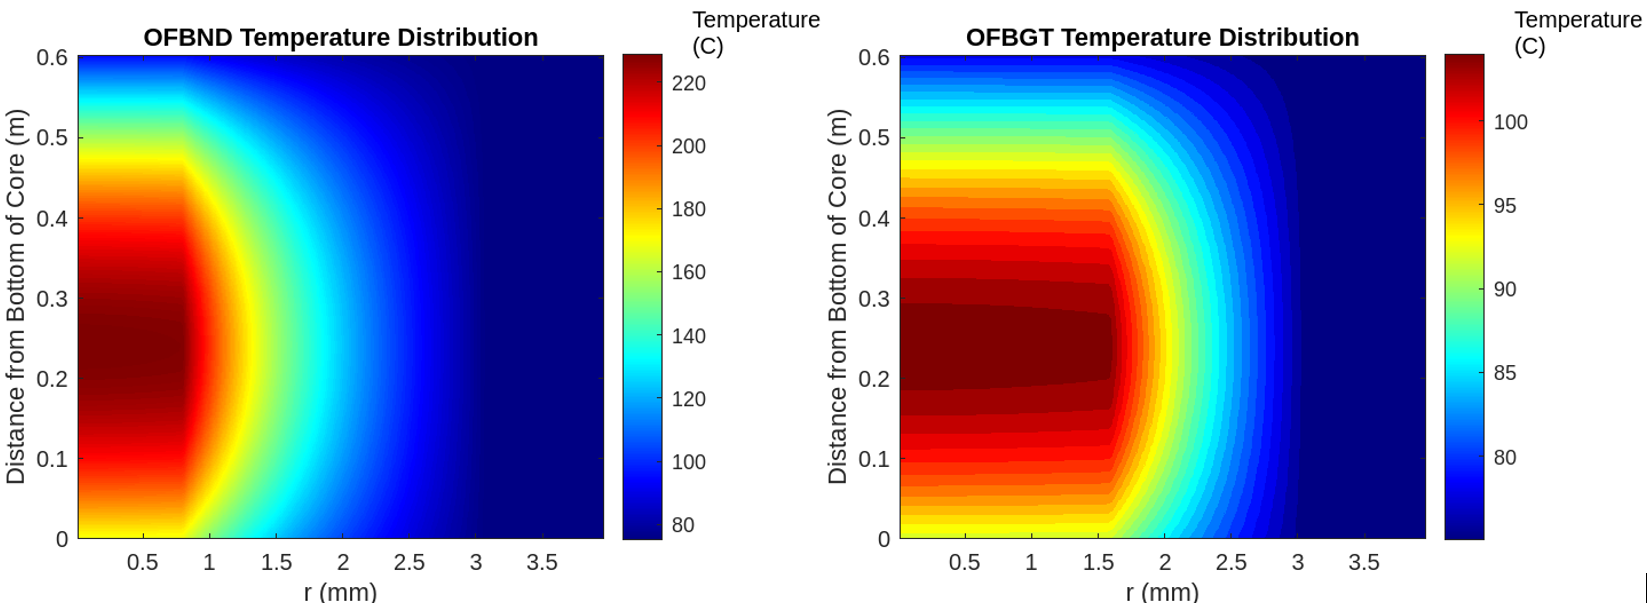
\includegraphics[width=0.85\textwidth]{figures/tempdist.png}
    \caption[Temperature distributions for the OFBGT and OFBND.]{Temperature distributions plotted as contour maps in the radial ($r$) and axial ($z$) directions for the OFBND (left) and the OFBGT (right).  The OFBND reaches significantly higher peak temperatures due to its larger linear power density.  Adapted from the OFBGT Simulation Response Document~\cite{SimReport2023}, p.~15.}
    \label{fig:temp_contour}
\end{figure}

\subsection{Modulation Transfer Function Results}

The normalized MTF curves for both the OFBGT and OFBND are compared in Figure~\ref{fig:MTF_comparison}.  The MTF quantifies the sensor's ability to faithfully reproduce axial variations in the energy deposition rate at different spatial frequencies.  A value of unity corresponds to perfect fidelity; lower values indicate spatial smoothing.

\begin{figure}[htbp]
    \centering
    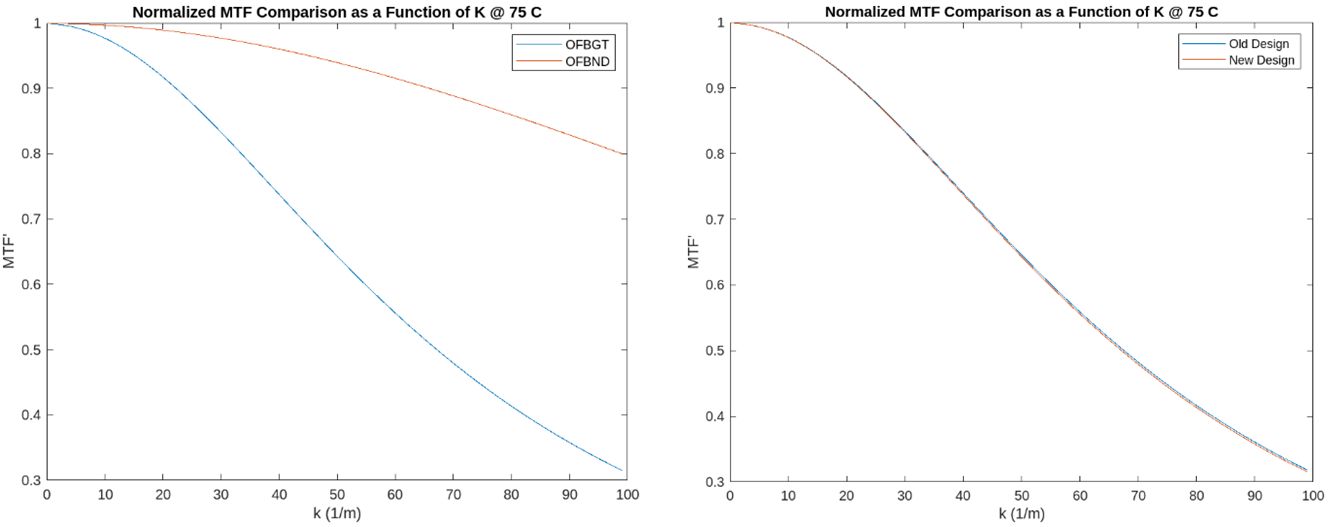
\includegraphics[width=0.85\textwidth]{figures/mft.png}
    \caption[Normalized MTF curves for the OFBGT and OFBND.]{Left: comparison of the normalized MTF curves for the OFBGT and OFBND as a function of spatial frequency $k$.  The OFBND exhibits a higher MTF at all spatial frequencies due to its smaller cross-sectional area and lower thermal mass conductivity.  Right: comparison of the new (Luna) OFBGT design with the original (Birri) OFBGT design, showing nearly identical MTF performance.  Adapted from the OFBGT Simulation Response Document~\cite{SimReport2023}, p.~16.}
    \label{fig:MTF_comparison}
\end{figure}

The OFBND exhibited a higher MTF at all spatial frequencies than the OFBGT.  This improved axial resolution is a consequence of the smaller cross-sectional area of the borosilicate glass thermal mass, which reduces the length scale over which axial thermal diffusion can smooth out spatial variations.  The MTF curves for the new (Luna) OFBGT design were found to be nearly identical to those of the original Birri design, confirming that the design modifications did not degrade the sensor's spatial resolution characteristics.

\section{Experimental Testing and Discussion of the OFBGT}
\label{sec:experimental_discussion}

\subsection{Reactor Testing Campaign}

Following the simulation work, an OFBGT was fabricated by Luna Innovations and tested in the CIF of the OSURR during a seven-hour reactor test campaign~\cite{LunaDOE2024}.  The sensor was equipped with ten FBG sensor pairs (inner and outer fiber) distributed along the 24-inch active sensor length.  The reactor was operated at multiple power levels (50\%, 70\%, 80\%, and 90\% of full power), and the temperature data from each FBG pair were recorded in real time.

\subsection{Discrepancy Between Predicted and Measured $\Delta T$}

The simulations presented in Section~\ref{sec:simulation_results} predicted a maximum $\Delta T$ of approximately 27--30~$^\circ$C for the OFBGT when deployed in the CIF at full reactor power, which exceeded the estimated measurement threshold of approximately 25~$^\circ$C needed for reliable power inference.  However, the experimental measurements yielded a significantly lower $\Delta T$, on the order of 17~$^\circ$C at full power.  This discrepancy rendered the $\Delta T$ insufficient for reliable calibration and power measurement, and the test was consequently deemed unsuccessful in meeting the original performance targets.

The primary source of the discrepancy was identified as the neglect of radiative heat transfer in the simulation models.  Both the Python and MATLAB models considered only conductive heat transfer through the gas gap.  However, at the operating temperatures of the thermal mass (approaching 100~$^\circ$C above ambient), radiative heat transfer across the gas gap between the thermal mass surface and the inner surface of the outer sheath provides a parallel pathway for heat dissipation that is not accounted for by conduction alone.  The radiative heat flux is governed by
\begin{equation}
    q''_\mathrm{rad} = \frac{\sigma (T_1^4 - T_2^4)}{\frac{1}{\varepsilon_1} + \frac{(1-\varepsilon_2)}{\varepsilon_2}\frac{r_{TM}}{r_{Si}}}
    \label{eq:radiative}
\end{equation}
where $\sigma$ is the Stefan--Boltzmann constant, $T_1$ and $T_2$ are the absolute temperatures of the thermal mass surface and the sheath inner surface, respectively, and $\varepsilon_1$ and $\varepsilon_2$ are the emissivities of these surfaces.

The inclusion of this radiative pathway effectively reduces the thermal resistance of the gas gap, lowering the equilibrium $\Delta T$.  The MATLAB code contained provisions for incorporating radiative heat transfer (with $\varepsilon_1 = 0.76$ for the mullite surface and $\varepsilon_2 = 0.05$ for the aluminum sheath), but this term was set to zero in the simulations presented in the response document based on the recommendation to neglect it at the time~\cite{SimReport2023}.  When radiative heat transfer was subsequently included in the model, the predicted $\Delta T$ dropped from approximately 27~$^\circ$C to approximately 17~$^\circ$C, in much closer agreement with the experimental observations.

This result underscores the importance of including all relevant heat transfer mechanisms, conduction, convection (if applicable), and radiation, in the thermal modeling of gamma thermometers, particularly when the gas gap temperature differential is large.  The lesson is especially pertinent for the OFBND, which operates at still higher temperatures and for which the neglect of radiative heat transfer would introduce even greater modeling errors.

\section{Status of the OFBND}
\label{sec:ofbnd_status}

The OFBND concept was investigated through simulation only during this research effort.  The modeling results predict a substantially larger $\Delta T$ (on the order of 155--159~$^\circ$C without radiative heat transfer corrections) for the OFBND in the AIF than for the OFBGT in the CIF, suggesting that the neutron dosimeter concept is viable from a signal-strength perspective.  The higher MTF of the OFBND further suggests superior axial resolution relative to the OFBGT.

However, no OFBND prototype has yet been fabricated or tested experimentally.  Several aspects of the OFBND design require experimental validation before the concept can be considered proven:

\begin{enumerate}
    \item \textbf{Thermal performance.}  The simulations predict operating temperatures in excess of 200~$^\circ$C in the thermal mass.  At such temperatures, radiative heat transfer, which was shown to be the dominant source of modeling error for the OFBGT, will be even more significant.  Updated simulations including radiative heat transfer are essential before a prototype is fabricated.
    \item \textbf{Material compatibility.}  The borosilicate glass thermal mass must survive prolonged exposure to the combined thermal, gamma, and neutron environment of the AIF without degradation in mechanical integrity or thermal properties.  The transmutation of boron-10 through the (n,$\alpha$) reaction will deplete the boron content over time, reducing the sensor's neutron sensitivity and introducing helium gas into the glass matrix.
    \item \textbf{Calibration methodology.}  The calibration of the OFBND with an internal heating wire is analogous to that of the OFBGT.  However, the separation of the neutron and gamma contributions to the measured $\Delta T$ requires a paired measurement with a collocated, purely gamma-sensitive OFBGT.  The practical feasibility of this approach remains to be demonstrated.
    \item \textbf{Signal-to-noise ratio.}  While the predicted $\Delta T$ is large, the FBG measurement uncertainty (typically $\pm 0.1$~$^\circ$C) must be small relative to the minimum resolvable $\Delta T$ at the lowest flux levels of interest.
\end{enumerate}

The OFBND therefore remains a promising but unproven concept that requires experimental testing to validate the theoretical predictions presented here.

\section{Summary}

This chapter has presented the simulation and analysis work performed in support of the OFBGT and OFBND sensor development.  The analytical thermal model, originally developed by Birri, was applied to a redesigned OFBGT intended for deployment in the CIF of the OSURR and extended to a neutron-sensitive variant (OFBND) intended for the AIF.

Two modeling approaches, a simplified Python model and an iterative MATLAB model with temperature-dependent thermal conductivities, yielded consistent predictions of $\Delta T$ for both sensors.  The simulations predicted a maximum $\Delta T$ of approximately 27--30~$^\circ$C for the OFBGT in the CIF and 155--159~$^\circ$C for the OFBND in the AIF, without accounting for radiative heat transfer.  The MTF analysis confirmed that both sensors possess adequate axial resolution for the spatial frequencies expected in the OSURR flux profiles, with the OFBND exhibiting superior resolution due to its smaller thermal mass.

Experimental testing of the OFBGT revealed that the measured $\Delta T$ was approximately 17~$^\circ$C, falling short of the approximately 25~$^\circ$C threshold required for reliable operation.  The discrepancy was attributed to the omission of radiative heat transfer in the original simulations.  When radiative heat transfer was included retrospectively, the model predictions agreed closely with the experimental observations.

The OFBND has not yet been fabricated or tested.  While the simulations indicate a favorable signal strength, experimental validation is required to confirm the thermal performance, material compatibility, and calibration methodology of the neutron dosimeter concept.  The inclusion of radiative heat transfer in future OFBND simulations is essential, given the high operating temperatures predicted for this sensor.